\documentclass[12pt]{article}
\usepackage{polski}
\usepackage[utf8]{inputenc}
\usepackage{amsmath}
\usepackage{anysize}
\usepackage{listings}
\lstset
{
	tabsize=2,
	breaklines=true,
	numbers=left,
	frame=single
}
\usepackage{graphicx}
\usepackage{color}
\title{Wykorzystanie silników fizycznych na platformach mobilnych}
\author{Mateusz Kortas}
\date{12.05.2012}
\begin{document}
\marginsize{2.5cm}{2cm}{1cm}{1cm}
  \maketitle
  \tableofcontents
  \section{Wstęp}\label{sec:wstep}
  \subsection{Czym jest silnik fizyczny?}\label{subsec:czymJestSilnik}
TODO
  \subsection{Cele projektu.}\label{subsec:celeProjektu}
TODO
  \section{Wykorzystane technologie.}
  \subsection{Android SDK}
TODO
  \subsection{Bullet physics engine}
TODO
Lorem Ipsum jest tekstem stosowanym jako przykładowy wypełniacz w przemyśle
poligraficznym. Został po raz pierwszy użyty w XV w. przez nieznanego drukarza do wypełnienia tekstem próbnej książki. Pięć wieków później zaczął być używany przemyśle elektronicznym, pozostając praktycznie niezmienionym. Spopularyzował się w latach 60. XX w. wraz z publikacją arkuszy Letrasetu, zawierających fragmenty Lorem Ipsum, a ostatnio z zawierającym różne wersje Lorem Ipsum oprogramowaniem przeznaczonym do realizacji druków na komputerach osobistych, jak Aldus PageMaker
  \subsection{Android NDK}
TODO
  \section{Wykorzystanie Bullet physics engine przez Android NDK}
  \subsection{Konfiguracja Android NDK w środowisku Eclipse}
  % [source]http://mhandroid.wordpress.com/2011/01/23/using-eclipse-for-android-cc-development/
  Aby utworzyć projekt Androida z możliwością edycji i kompilacji bibliotek
  natywnych należy: \\
  1. Zainstalować środowisko Eclipse(i doinstalować do niego wtyczkę
  \emph{ADT}).\\
  2. Pobrać kolejno Android SDK i NDK. Do edycji plików żródłowych jest
  też konieczne pobranie wtyczki \emph{CDT}(C++ Development Tools). Potrzebny
  będzie rónież kod żródłowy biblioteki bullet. Dodatki w eclipse instaluje się przez
  Help -> Install new software\ldots , wpisując adres http://download.eclipse.org/releases/galileo (lub zamisat
  galileo wpisać nazwę swojej wersji Eclipse).
  
  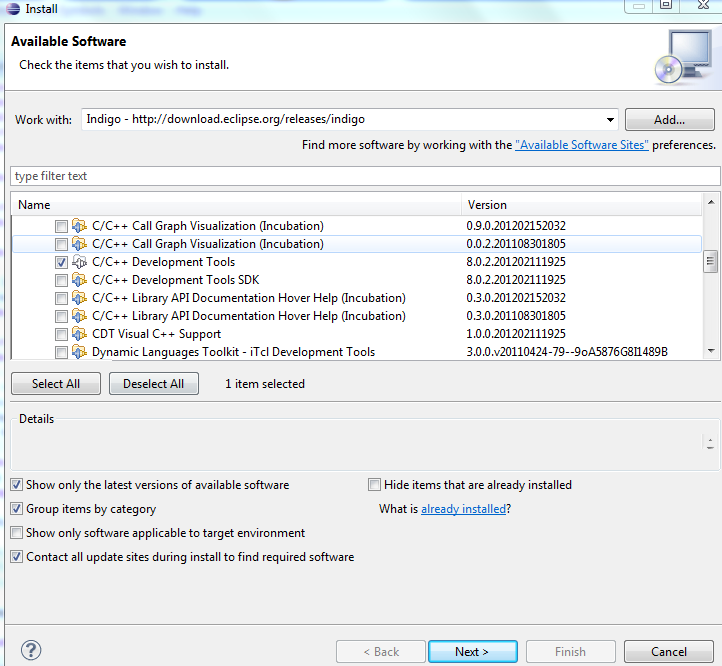
\includegraphics[width=\textwidth]{./img/CDT.png}
  3. Utworzyć nowy standardowy projekt aplikacji na system Android.\\
  4. Do projektu dodać folder \emph{jni} gdzie przechowywany będzie kod źródłowy
  w języku C++. Skopiować do niego foldery z kodu źródłowego biblioteki
  bullet(będą potrzebne biblioteki BulletCollision, BulletDynamics i
  LinearMath, a także pliki btBulletCollisionCommon.h,
  btBulletDynamicsCommon.h, Bullet-C-Api.h).
  
  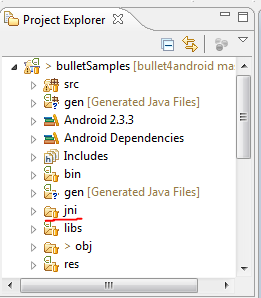
\includegraphics{./img/jni-folder.png}
  
  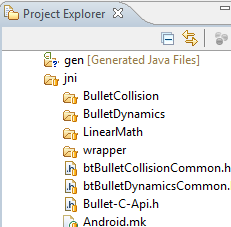
\includegraphics{./img/bulletFoldery.png}
  
  5. Umieścić w folderze plik Android.mk . Zawiera on informacje jak powinien
  być zbudowany projekt w kodzie natywnym. Do tego pliku należy
  dodać informacje o plikach źródłowych biblioteki bullet.
  \lstinputlisting[language=make, caption=Zawartość pliku Android.mk,
  label=andMake,
  breaklines=true,numbers=left,frame=single]{./listings/bulletMkfile.mk}
  
  6. Przekonwertować projekt java na java/C++ , przez menu File -> New ->
  Other\ldots
  
  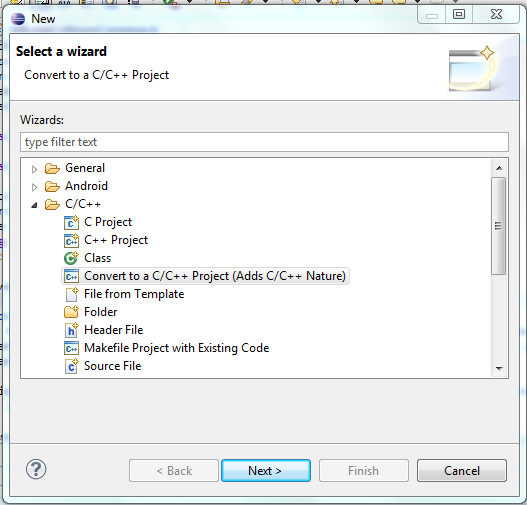
\includegraphics{./img/convert.png}
  
  7. W Properties projektu ustawić budowanie kodu w C++ przez ndk-build.
  Najlepiej miejsce rozpakowania Android NDK przypisać pod zmienną środowiskową
  (np. NDKROOT), co ułatwi przenośność projektu.
  
  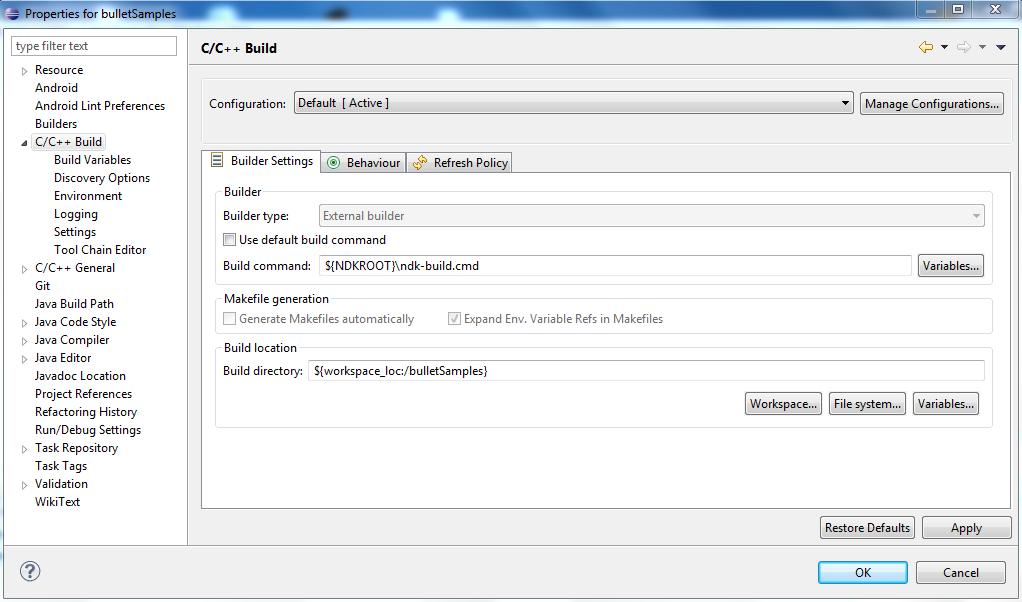
\includegraphics[width=\textwidth]{./img/properties.png}
  
  W zakładce behavior należy odznaczyć checkboxa Clean i usunąć tekst z pola
  Build.\\
  8. W C++ General -> Paths And Symbols dodać ścieżkę dla nagłówków.
 
  9. Ponieważ w projekcie będą wykorzystywane elementy biblioteki STL, konieczne
  jest dodanie odpowiedniej ścieżki.\\
  
  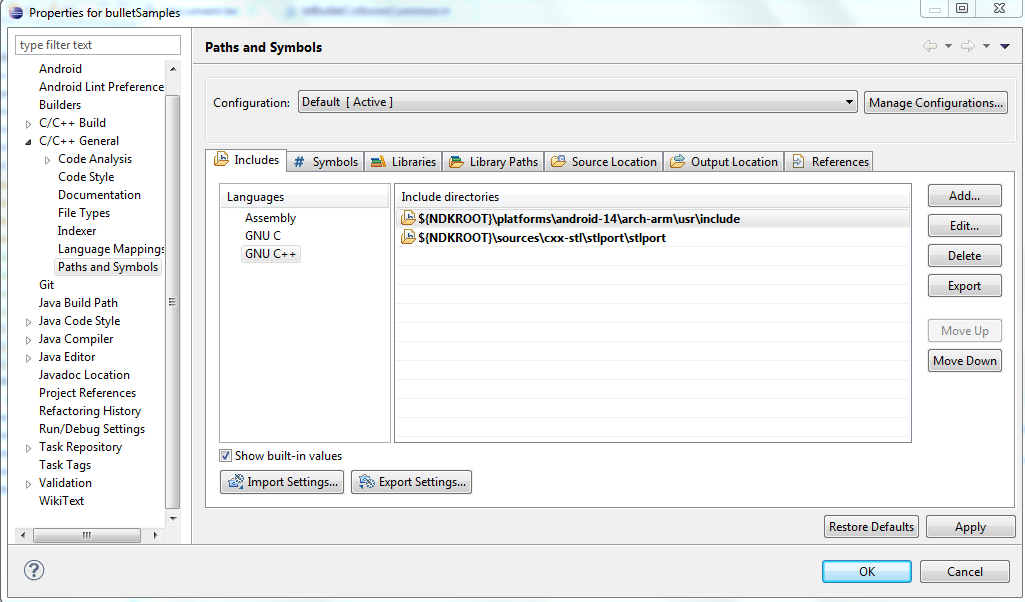
\includegraphics[width=\textwidth]{./img/ndkroot.png}
  
  Dodać również należy informację o wykorzystaniu STL w pliku
  Application.mk(który również muisi być dodany do projektu).
  
  \lstinputlisting[language=make, caption=Zawartość pliku Application.mk,
  label=andMake]{./listings/Application.mk}
  
  Po tych czynnościach można edytować projekt ze składnią Javy jak i C++,
  korzystając z autouzupełniania i jednolitej kompilacji. Należy jednak
  pamiętać, że przy dodawaniu nowego pliku z kodem źródłowym w C++ do folderu
  \emph{jni} konieczne jest umieszczenie o nim informacji w Android.mk .

\subsection{Wywoływanie funkcji natywnych z poziomu Javy}

\subsection{Konserwacja obiektów}

\subsection{Przekazywanie argumentów i zwracanych wartości}

\section{Wykorzystanie silnika Bullet w doświadczeniach fizycznych}

\subsection{Gromadzenie pomiarów}
W celu łatwego gromadzenia danych pomiarowych w trakcie trwania testu powstała
klasa Logger przechowująca funkcje odpowiadające za przechowywanie danych w
pamięci urządzenia.
  \lstinputlisting[language=Java, caption=Klasa Logger,
  label=lis:logger]{./listings/Logger.java}
Należy również pamiętać o zezwoleniu aplikacji na manipulowanie pamięcią
zewnętrzną. Konieczny jest wpis w manifeście aplikacji.
\lstinputlisting[language=xml, caption=zawartość pliku AndroidManifest.xml,
  label=lis:manifest,linerange={6-9}]{./listings/AndroidManifest.xml}

\subsection{Zasada zachowania energii}

\subsubsection{Przypadek z jednym ciałem}
Na początek zostanie rozważony najprostszy przypadek z jedną kulką odbijającą
się kolejno od dwóch idealnie sprężystych ścianek. Do tego testu wykorzystana
została scena prezentowana na listingu \ref{lis:SimpleSnookerScene}.
 \lstinputlisting[language=Java,
caption=scena testująca przypadek z jednym ciałem,
label=lis:SimpleSnookerScene]{./listings/SimpleSnookerScene.java}
Na niesprężystym podłożu(ln. 57) zostaje umieszczona kulka(ln. 59), która przez
nadaną jej prędkość początkową(ln. 62) odbija się kolejno od ścianek(ln. 49,
50). Sprężystość(\emph{restitution}) kulki jak i ścianek jest regulowana na
początku każdego testu(ln. 73, 74), która dla pierszego wynosi 0.9(ln. 18) i
jest liniowo zwiększana dla kolejnych dziesięciu testów(ln. 21, 24, 94) aż do
osiągnięcia wartości 1(gdzie teoretycznie energia kulki powinna być stała).
Dla każdej testowanej wartości przewidziano 20 odbić(ln. 22, 23, 81-97). Energia
kinetyczna kulki jest zapisywana do pliku przy każdym odbiciu(ln. 81-87).

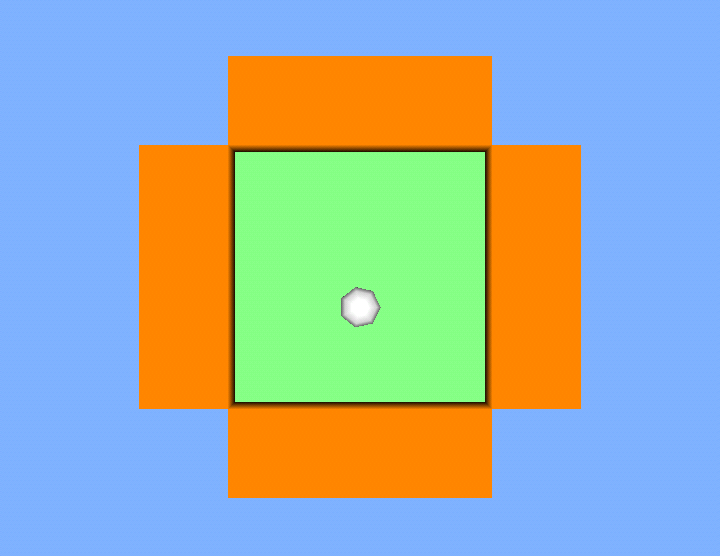
\includegraphics[width=\textwidth]{./img/SimpleSnookerScene.png}

Zależność energii kinetycznej kulki przy kolejnych jej odbiciach od wartości
sprężystości jest przedstawiona na poniższym wykresie.

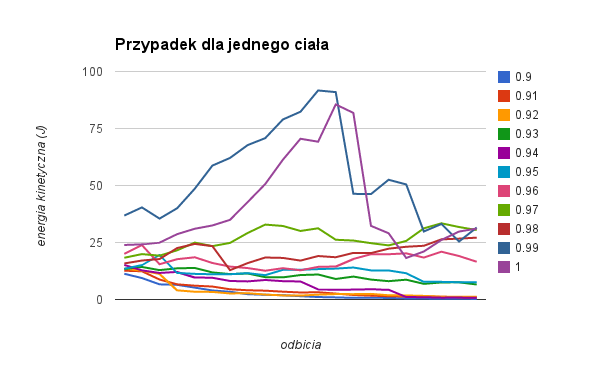
\includegraphics[width=\textwidth]{./img/chart_1.png}

Jak widać w doświadczeniu nie osiągnięto spodziewanych rezultatów. Dla
sprężystości o wartości 1 energia kinetyczna powinna być stała, natomiast tutaj
gwałtownie wzrasta. Wydaje się, że dla utrzymania stałej energii kinetycznej
konieczne jest użycie niższej wartości. Dla polepszenia widoczności poniższy
wykres zawiera wartości energii kinetycznej dla wartości sprężystości od 0,94 do
0,98.

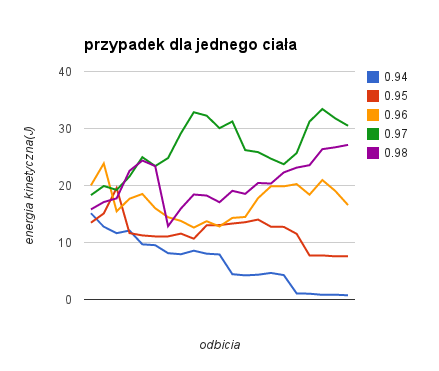
\includegraphics{./img/chart_2.png}

Przy początkowej prędkości 5 m/s i masie 1 kg (linting
\ref{lis:SimpleSnookerScene} ln. 72, 59) energia kinetyczna kulki powinna mieć
stałą wartość energii kinetycznej 12,5.
TODO równanie obliczenia EK.
Z prezentowanego wykresu wynika, że najodpowiedniejsza wartość współczynnika
sprężystości kulki i ścianek mieści się między 0,95 a 0,96.//
Dla ustalenia bardziej szczegółowej wartości test został powtórzony dla
następujących parametrów z listingu \ref{lis:SimpleSnookerScene}:

\lstinputlisting[language=Java,
  label=lis:SimpleSnookerScene_additional]{./listings/SimpleSnookerScene_additional.java}
  
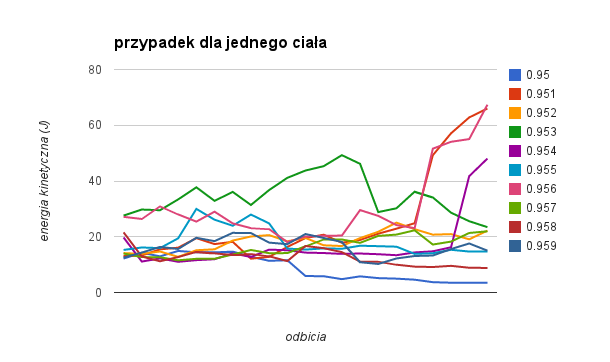
\includegraphics[width=\textwidth]{./img/chart_3.png}

Jak widać w otrzymywanej energii kinetycznej występuje spory wkład losowości.
Oceniając jednak wynik testu można stwierdzić, że najbardziej odpowiednią
wartością dla współczynnika sprężystości jest 0,955 ponieważ wartość energii
kinetycznej przy ostatnim zarejestrowanym odbiciu dla tego współczynnika(14,74)
była najbliżasza wartości spodziewanej(12,5).
  
\end{document}
%http://java.sun.com/docs/books/jni/html/refs.html

%przelatywanie przez bandę - zabawa parametrami
%zderzenie 2 kulek - zachowana energia?
%zderzenie 3 kulek - czy jest rozpatrywane poprawnie
%jelly i newtonPendulum - zachowalność energii
%rotacja kulki - czy przy dużych obrotach będzie się cofać przy odbijaniu
%edoświadczenia